\documentclass[a4paper,12pt]{article}
 \usepackage[utf8]{inputenc}
 \usepackage[left=2cm,top=1cm,right=2cm,bottom=1.5cm,nohead]{geometry}
%\usepackage{wrapfig} % Обтекание рисунков текстом
%\usepackage{floatflt}% Обтекание таблиц текстом
 \usepackage{amsmath} % Математические окружения AMS
 \usepackage{amsfonts} % Шрифты AMS
 \usepackage{amssymb} % Символы AMS
 \usepackage{listings}% to add computer code
 \usepackage{color}
 \definecolor{mygreen}{RGB}{28,172,0} % color values Red, Green, Blue
\definecolor{mylilas}{RGB}{170,55,241}
    \usepackage{graphicx} % Вставить pdf- или png-файлы
  \usepackage{euscript} % Красивый шрифт
%\usepackage{extsizes} % Возможность сделать 14-й шрифт
 \linespread{1.5} % Интерлиньяж
% \usepackage[usenames,dvipsnames,svgnames,table,rgb]{xcolor}% чтоб были гиперссылки и чтоб были цвета

\usepackage{hyperref} % Гиперссылки

%\hypersetup{
% colorlinks = true,
 %linkcolor = MidnightBlue, % ссылки на всякие разделы (их цвет)
 %urlcolor = [rgb]{0,0,1}, % чтоб задавать цыета пиксела - red green blue. не рекомендуется, если потом печатать.
 %citecolor = black
%}
%\usepackage{pdflscape}
%\oddsidemargin=10mm
%\topmargin=-15mm
\usepackage{multicol}
%\hoffset=5mm % см при печати
%\voffset=4.2mm
%\textheight = 720pt
%\textwidth=442pt

\begin{document}
\maketitle \hrulefill
\lstset{language=Matlab,%
    %basicstyle=\color{red},
    breaklines=true,%
    morekeywords={matlab2tikz},
    keywordstyle=\color{blue},%
    morekeywords=[2]{1}, keywordstyle=[2]{\color{black}},
    identifierstyle=\color{black},%
    stringstyle=\color{mylilas},
    commentstyle=\color{mygreen},%
    showstringspaces=false,%without this there will be a symbol in the places where there is a space
    numbers=left,%
    numberstyle={\tiny \color{black}},% size of the numbers
    numbersep=9pt, % this defines how far the numbers are from the text
    emph=[1]{for,end,break},emphstyle=[1]\color{red}, %some words to emphasise
    %emph=[2]{word1,word2}, emphstyle=[2]{style},
}

\begin{center}

\textbf {\Large{Empirical Methods HA 3}}\\
Konstantin Guryev\\
Pennsylvania State University\\
2018
\end{center}

\textbf{Problem \textnumero \,1 }

\vspace{\baselineskip}
$\beta_{mle}$
 =
\begin{pmatrix}
  2.5339 \\
  -0.0323\\
  0.1157\\
  -0.3540\\
  0.0798\\
  -0.4094
\end{pmatrix};
\vspace{\baselineskip}

\textbf{Problem \textnumero \,2 }

\vspace{\baselineskip}
$\beta_{mleqn}$
 =
\begin{pmatrix}
 2.5339 \\
  -0.0323\\
  0.1157\\
  -0.3540\\
  0.0798\\
  -0.4094
\end{pmatrix};
\vspace{\baselineskip}

\textbf{Problem \textnumero \,3 }

\vspace{\baselineskip}
$\beta_{nls}$
 =
\begin{pmatrix}
 2.5126 \\
  -0.0384\\
  0.1141\\
  -0.2796\\
  0.0676\\
  -0.3698
\end{pmatrix};
\vspace{\baselineskip}

\textbf{Problem \textnumero \,4 }

\vspace{\baselineskip}
$\beta_{nlsnm}$
 =
\begin{pmatrix}
  2.5126 \\
  -0.0384\\
  0.1141\\
  -0.2796\\
  0.0676\\
  -0.3698
\end{pmatrix};
\vspace{\baselineskip}

\textbf{Problem \textnumero \,5 }

\vspace{\baselineskip}
By looking on the graph we may conclude that MLE via the Nelder-Mead is the slowest method, then comes the NLS (lsqonlin) method. And MLE via a quasi-Newton and NLS via Nelder-Mead are the fastest ones. 

\begin{figure}[h]
\centering
%\begin{center}
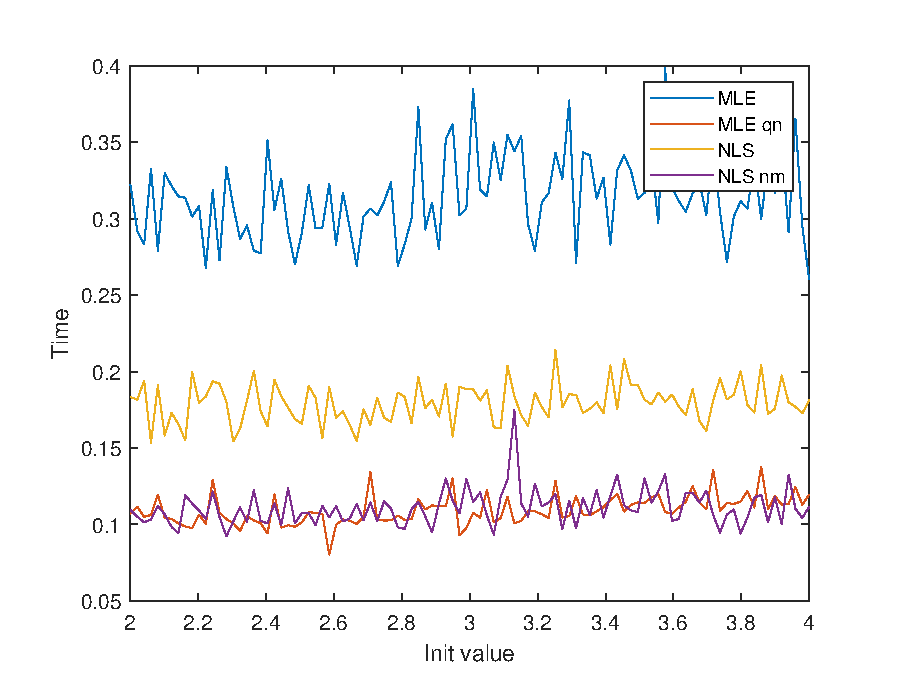
\includegraphics[width=16cm,height=8cm,keepaspectratio]{fig1.eps}
%\caption{Движущийся жесткий штамп}
%\caption{pic1}
%\end{center}
\end{figure}
\vspace{\baselineskip}

\newpage
\section*{Matlab Code} \lstinputlisting{likelihood1.m}
\newpage
\section*{Matlab Code} \lstinputlisting{likelihood2.m}
\newpage
\section*{Matlab Code} \lstinputlisting{mle_est.m}
\newpage
\section*{Matlab Code} \lstinputlisting{mle_qn_est.m}
\newpage
\section*{Matlab Code} \lstinputlisting{nls_est.m}
\newpage
\section*{Matlab Code} \lstinputlisting{nls_nm_est.m}
\newpage
\section*{Matlab Code} \lstinputlisting{HA_3_Guryev.m}


\end{document}
